\begin{figure}[t]
  \centerline{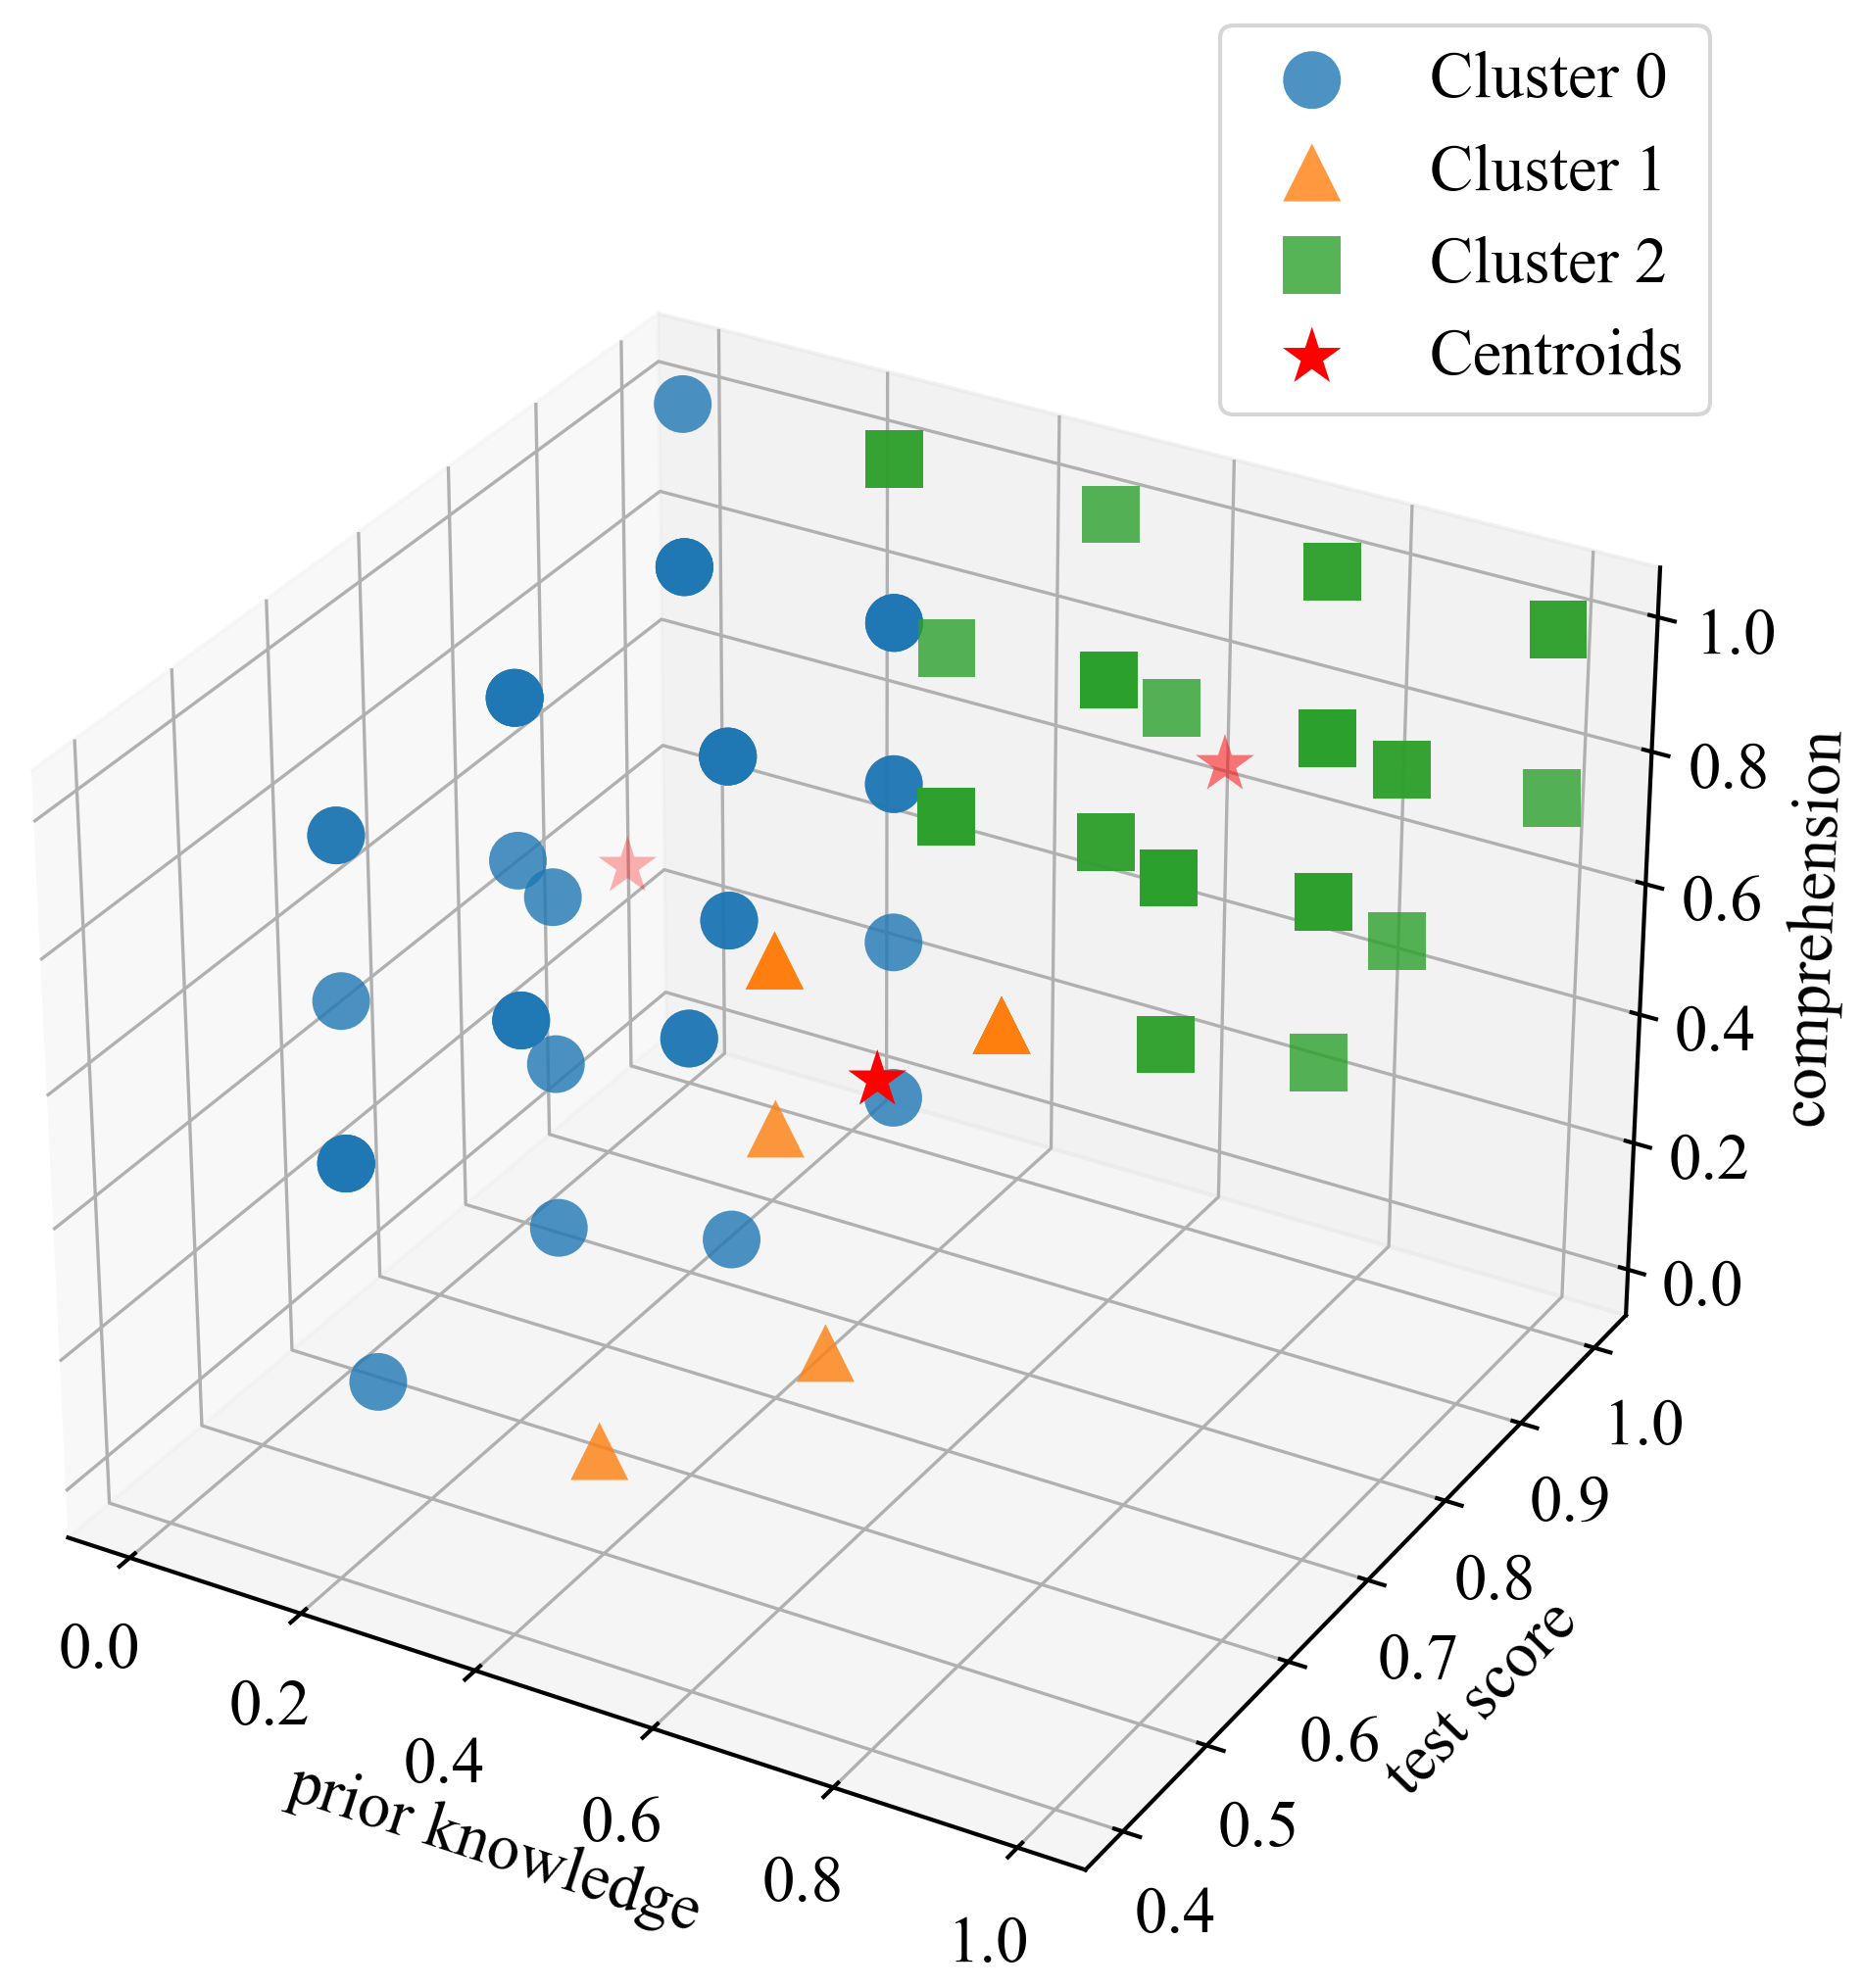
\includegraphics[width=\linewidth]{img/kmeans.png}}
  \caption{K-means result}
  \label{k-means_train}
\end{figure}

%1st paragraph
% 活動レベルの位置づけ
The activity levels were treated as a measure that integrates the subjective and objective perspectives.
  %
  The two indicators were converted into numerical labels by clustering.
  %
  The labels were defined as the group labels (GL).
    %
    GL represents the clustering results that capture multiple activity levels.
% k-meansの手順
K-means was used as a clustering method to split samples into $k$ groups \cite{krishna1999genetic}.
  %
  The number of clusters was set to $k=3$.
% k-meansの結果
Fig.~\ref{k-means_train} shows the clustering results.
% 点群データセットへのGLの割り当て
A GL cluster was assigned to each point-cloud dataset as an activity-level indicator.

%2nd paragraph
% データ拡張の実施
Data extension was performed to increase the available data samples.
\revised{Data extension compensated for the limited number of point-cloud datasets.
Public datasets combining video viewing and test-taking are unavailable.}
% データ拡張の方法
The datasets were extended by generating pairs of point-cloud datasets based on relational similarity~\cite{shinkuma2019relational}.
  % ペアの生成
  The point-cloud dataset pairs were formed from the $N=110$ point-cloud datasets ($\binom{N}{2}=5995$ pairs) without duplication.
  % ペアの特徴ベクトル間の絶対差分の計算
  The input features were computed as the element-wise absolute value of the difference between the feature vectors of each of the point-cloud dataset pairs.

%3rd paragraph
% MLの定義
Agreement and disagreement between the GL of the two datasets in each of the point-cloud datasets pairs are defined as matching labels (ML).
  % MLの形式
  ML is represented as a binary label.
\revised{Dataset pairs enabled supervised comparison of feature-vector differences between sessions with known GL relationships.}
